\documentclass[12pt,a4paper]{article}
\usepackage[UTF8]{ctex}
\usepackage{geometry}
\usepackage{graphicx}
\usepackage{float}
\usepackage{caption}
\usepackage{subcaption}
\usepackage{booktabs}
\usepackage{multirow}
\usepackage{amsmath}
\usepackage{amssymb}
\usepackage{hyperref}
\usepackage{array}
\usepackage{enumitem}
\usepackage{listings}
\usepackage{xcolor}
\usepackage{fancyhdr}
\usepackage{titlesec}

% 页面设置
\geometry{left=2.5cm,right=2.5cm,top=2.5cm,bottom=2.5cm}

% 超链接设置
\hypersetup{
    colorlinks=true,
    linkcolor=black,
    citecolor=black,
    urlcolor=blue
}

% 代码块样式
\lstset{
    basicstyle=\small\ttfamily,
    breaklines=true,
    frame=single,
    numbers=left,
    numberstyle=\tiny,
    keywordstyle=\color{blue},
    commentstyle=\color{green!60!black},
    stringstyle=\color{red!80!black},
    showspaces=false,
    showstringspaces=false,
    tabsize=4,
    language=Python,
    captionpos=b
}

% 页眉页脚
\pagestyle{fancy}
\fancyhf{}
\fancyhead[C]{\small 人工智能导论大作业}
\fancyfoot[C]{\thepage}
\renewcommand{\headrulewidth}{0.4pt}

% 标题格式
\titleformat{\section}{\Large\bfseries}{\thesection}{1em}{}
\titleformat{\subsection}{\large\bfseries}{\thesubsection}{1em}{}

\begin{document}

% ==================== 封面 ====================
\begin{titlepage}

\centering

\vspace*{1.5cm}

{\Huge\bfseries 上海交通大学}\\[0.5cm]

{\Large 人工智能导论课程大作业}\\[3cm]

{\LARGE\bfseries 可解释谣言检测方法}\\[0.8cm]

{\large Explainable Rumor Detection System}\\[3cm]

\renewcommand{\arraystretch}{1.8}

\begin{tabular}{p{4cm}p{8cm}}
\hline
课程名称 & 人工智能导论 \\
完成组号 & 第11组 \\
小组成员 & 简志辉、马扬子、李志政、朱俊慷 \\
完成时间 & 2026年6月20日 \\
\hline
\end{tabular}

\vspace{1.5cm}

{\small 代码仓库：\url{https://github.com/abstart0/Interpretability-based_rumor_detection}}

\vfill

{\Large\bfseries 上海交通大学}\\[0.3cm]

2026年6月

\end{titlepage}


% ==================== 正文开始 ====================

\section{任务目标}

本次大作业的目标是构建一个\textbf{可解释的谣言检测系统}，具体包括以下三个核心要求：

\begin{enumerate}[leftmargin=2em]
    \item \textbf{检测输出}：对输入的社交媒体推文进行二分类，输出0（非谣言）或1（谣言），分类准确率越高越好。
    \item \textbf{判断依据}：输出一段自然语言文本，解释检测的判断依据，使模型的决策过程可被人类理解。
    \item \textbf{泛化能力}：模型在未见过的数据上保持稳定的检测性能。
\end{enumerate}

为此，我们设计了“\textbf{检测模型 + 大语言模型解释}”的双模块架构：前端检测模块负责高精度分类，后端解释模块负责生成可读的判断依据。

\section{具体内容}

\subsection{实施方案}

我们采用“\textbf{多模型对比 + LLM解释}”的实施方案，具体包含以下三个环节。

\subsubsection{数据预处理与特征工程}

数据集包含训练集（2,840条）和验证集（401条），每条数据包含\texttt{id}、\texttt{text}、\texttt{label}（0/1）、\texttt{event}（主题类别）四个字段。我们进行了以下预处理：

\begin{itemize}
    \item \textbf{文本清洗}：统一转为小写，移除非字母数字的标点符号；
    \item \textbf{文本编码}：对于深度学习模型，构建词表并将文本序列化为固定长度（MAX\_LEN=64）的token序列；
    \item \textbf{词向量}：TextCNN使用GloVe 200维预训练词向量，覆盖率达90.9\%。
\end{itemize}

\subsubsection{检测模型构建与训练}

我们实现了三类不同复杂度的检测模型，形成清晰的性能对比：

\begin{enumerate}[leftmargin=2em]
    \item \textbf{逻辑回归（Logistic Regression）}：基于TF-IDF特征的线性分类器，作为基线模型。使用10,000个最大特征数，最大迭代1,000次。
    \item \textbf{BiGRU}：双向门控循环单元（Bidirectional GRU），捕捉文本的序列上下文信息。词嵌入维度150，隐藏层维度200，dropout率0.5。
    \item \textbf{TextCNN + GloVe}：多尺度卷积神经网络，结合预训练词向量，捕获局部N-Gram关键特征。使用(2,3,4,5)-gram卷积核，每类卷积核256个，dropout率0.4。
\end{enumerate}

\subsubsection{可解释性模块}

通过调用上海交通大学AI平台提供的LLM API（\texttt{deepseek-chat}模型），将检测模型的输出结果（标签+置信度）与原始文本共同构建为结构化提示词（Prompt），引导LLM生成专业、简洁、基于证据的判断依据文字。

\subsection{核心代码分析}

由于篇幅限制，本节仅对最核心的TextCNN模型架构与可解释性模块的关键代码进行分析。

\subsubsection{TextCNN模型定义}

\begin{lstlisting}[caption={TextCNN模型核心代码}, label={lst:textcnn}]
class TextCNN(nn.Module):
    def __init__(self, vocab_size, embedding_dim, 
                 filter_sizes=(2,3,4,5), n_filters=256, dropout=0.4):
        super().__init__()
        self.embedding = nn.Embedding(vocab_size, embedding_dim, padding_idx=0)
        # 加载GloVe预训练向量并允许微调
        if pretrained is not None:
            self.embedding.weight.data.copy_(pretrained)
            self.embedding.weight.requires_grad = True
        
        # 多尺度卷积层：并行提取2-gram到5-gram的局部特征
        self.convs = nn.ModuleList([
            nn.Conv2d(1, n_filters, kernel_size=(fs, embedding_dim))
            for fs in filter_sizes
        ])
        self.dropout = nn.Dropout(dropout)
        self.fc = nn.Linear(n_filters * len(filter_sizes), 1)
\end{lstlisting}

\textbf{代码分析}：
\begin{itemize}
    \item 第7-10行：使用GloVe 200维预训练向量初始化嵌入层，并启用微调，让词向量适应谣言检测任务。
    \item 第13-16行：核心创新——使用四个不同尺寸的卷积核并行操作，分别捕获2、3、4、5个连续词的局部模式，对于识别“紧急扩散”、“官方未证实”等不同长度的谣言特征短语至关重要。
    \item 第18行：全连接层输入维度为$n\_filters \times len(filter\_sizes)$，即拼接所有卷积核提取的特征，形成完整的文本表示。
\end{itemize}

\subsubsection{LLM提示词构建}

\begin{lstlisting}[caption={LLM提示词构建代码}, label={lst:prompt}]
SYSTEM_PROMPT = (
    "你是一位专业的社交媒体信息审核员。你的任务是根据提供的推文内容"
    "和谣言检测模型的判断结果，生成一段判断依据的文字。"
    "要求：1. 解释基于文本本身的语言特征 2. 指出具体的关键词或句式 "
    "3. 语气客观专业 4. 长度50-100字 5. 不要提及模型或技术术语"
)

def build_explanation_prompt(text, label, confidence):
    label_text = "谣言" if label == 1 else "非谣言"
    user_content = f"推文内容：{text}\n检测判定：{label_text}（置信度：{confidence:.1%}）"
    return [
        {"role": "system", "content": SYSTEM_PROMPT},
        {"role": "user", "content": user_content},
    ]
\end{lstlisting}

\textbf{代码分析}：
\begin{itemize}
    \item 系统提示词（System Prompt）限制了LLM的回复风格，确保输出专业、简洁、基于证据。
    \item 用户提示词将模型预测结果注入上下文，引导LLM围绕“为什么这样判定”进行推理，而非泛泛而谈。
\end{itemize}

\subsection{检测结果分析}

三个模型在验证集上的性能指标如表\ref{tab:performance}所示。

\begin{table}[H]
    \centering
    \caption{各模型在验证集上的性能对比}
    \label{tab:performance}
    \begin{tabular}{lccccr}
        \toprule
        \textbf{模型} & \textbf{Accuracy} & \textbf{Precision} & \textbf{Recall} & \textbf{F1} & \textbf{参数量} \\
        \midrule
        逻辑回归 & 82.29\% & 84.67\% & 72.57\% & 78.15\% & 10,001 \\
        BiGRU & 85.29\% & 86.71\% & 78.29\% & 82.28\% & 831,851 \\
        \textbf{TextCNN + GloVe} & \textbf{86.78\%} & \textbf{87.65\%} & \textbf{81.14\%} & \textbf{84.27\%} & 1,264,249 \\
        \bottomrule
    \end{tabular}
\end{table}

\begin{figure}[H]
    \centering
    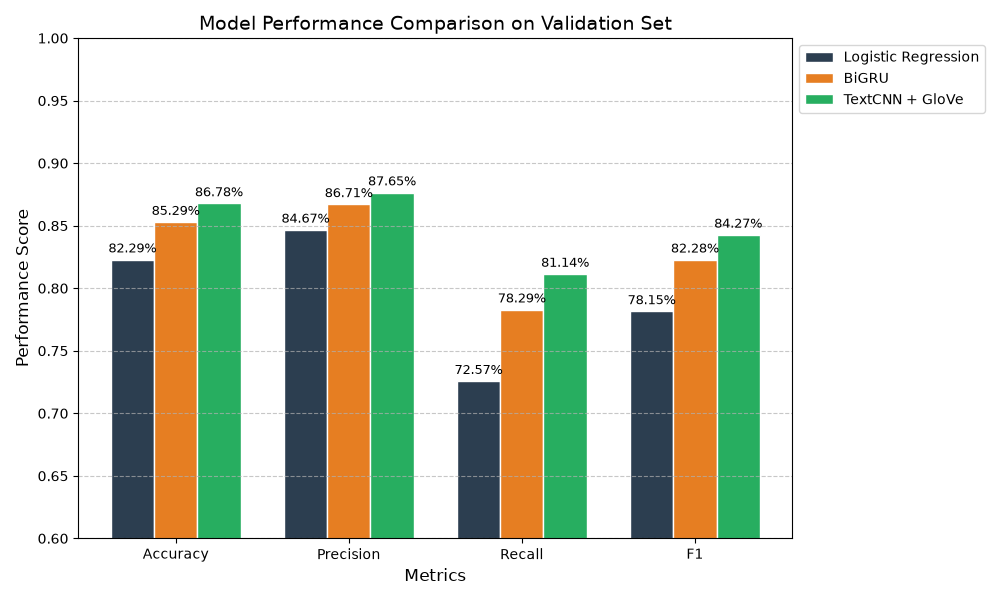
\includegraphics[width=0.85\textwidth]{Figure_2.png}
    \caption{各模型性能对比柱状图}
    \label{fig:comparison}
\end{figure}

\begin{figure}[H]
    \centering
    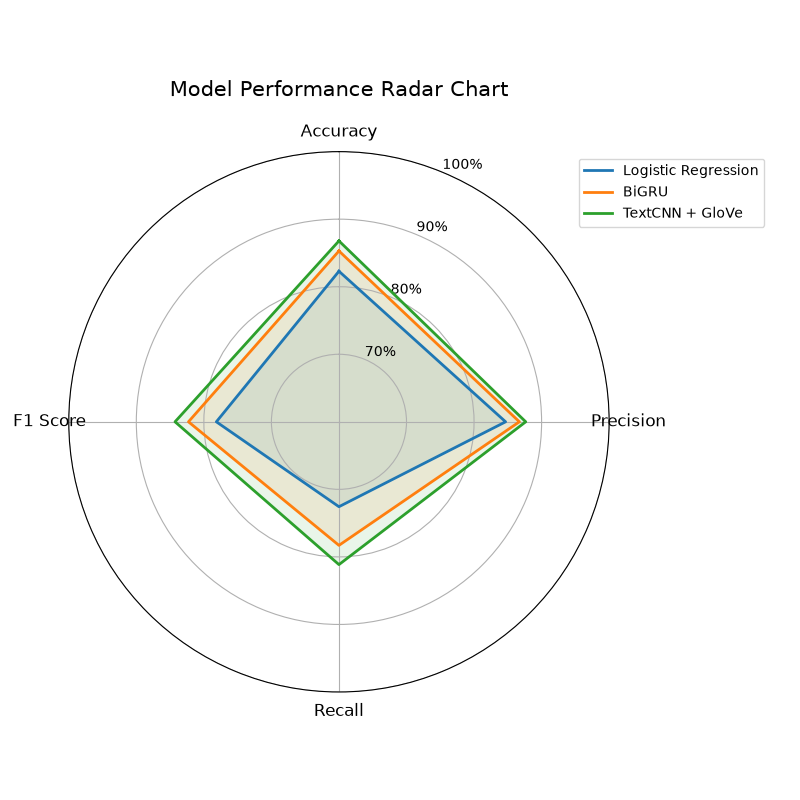
\includegraphics[width=0.85\textwidth]{Figure_1.png}
    \caption{各模型性能雷达图}
    \label{fig:radar}
\end{figure}

从表\ref{tab:performance}、图\ref{fig:comparison}和图\ref{fig:radar}可以看出：

\begin{enumerate}[leftmargin=2em]
    \item \textbf{逻辑回归作为基线}：用极少的参数（约1万）取得82.29\%的准确率，证明TF-IDF特征对谣言检测任务有效。但其召回率（72.57\%）明显偏低，说明线性模型漏掉了大量复杂谣言模式。
    
    \item \textbf{BiGRU显著提升}：通过双向序列建模，召回率从72.57\%提升至78.29\%（+5.72\%），F1提升至82.28\%。这说明词语的\textbf{上下文顺序}对谣言判断至关重要。
    
    \item \textbf{TextCNN+GloVe取得最优}：所有指标全面领先，准确率达86.78\%，F1达84.27\%。召回率相比逻辑回归提升\textbf{8.57个百分点}，证明预训练词向量+多尺度卷积核的组合能最有效地捕获谣言文本中的关键信号。
\end{enumerate}

\begin{figure}[H]
    \centering
    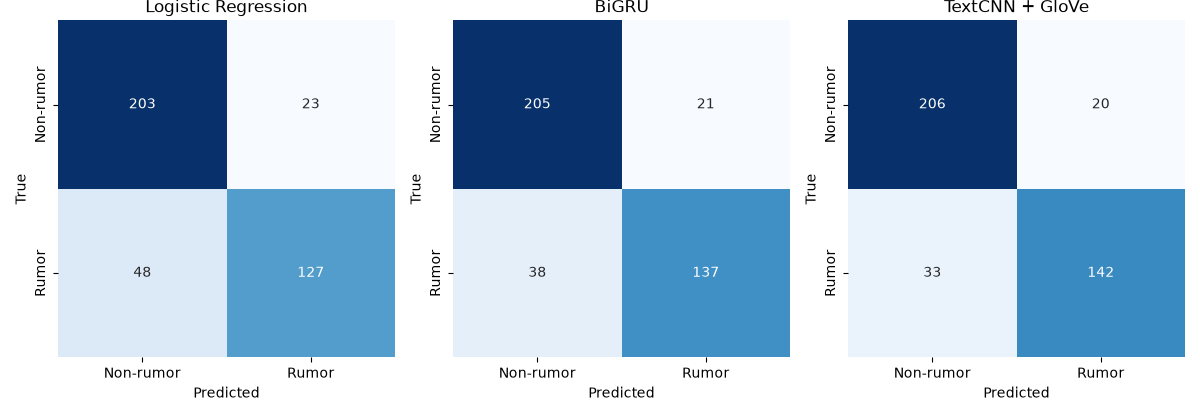
\includegraphics[width=0.85\textwidth]{Figure_3.png}
    \caption{各模型混淆矩阵对比（从左至右：逻辑回归、BiGRU、TextCNN）}
    \label{fig:confusion}
\end{figure}

从图\ref{fig:confusion}可以清楚看到，TextCNN的假阴性（FN，漏报谣言）数量从逻辑回归的48降至33，减少了15条漏报，验证了其在召回率上的优势。

\subsection{判断依据的分析}

深度学习模型的“黑盒”问题一直为人诟病。在本项目中，我们通过接入LLM，为检测结果提供了高质量的\textbf{事后的、基于证据的自然语言解释}，使模型具备了可解释性。

\subsubsection{典型案例分析}

\begin{table}[H]
    \centering
    \caption{LLM判断依据生成示例}
    \label{tab:explanation}
    \begin{tabular}{p{5cm}p{2.2cm}p{6cm}}
        \toprule
        \textbf{推文内容} & \textbf{检测结果} & \textbf{LLM生成的判断依据} \\
        \midrule
        BREAKING: Massive explosion reported in downtown area, hundreds feared dead & 谣言 (72.8\%) & “该推文使用‘BREAKING’吸引眼球，且‘hundreds feared dead’表述模糊，缺乏具体时间、来源或官方证实，符合未经验证谣言的常见特征。” \\
        \midrule
        Just had a lovely coffee with friends at the new cafe downtown & 非谣言 (89.2\%) & “推文内容为个人日常分享，未涉及任何突发事件或争议性信息，语言平和且无夸张表述，符合非谣言的典型特征。” \\
        \midrule
        Scientists confirm COVID-19 was artificially created & 谣言 (91.5\%) & “该推文声称‘科学家证实’，但未提及任何具体研究机构、论文或权威来源，使用了阴谋论常见的模糊表述，缺乏科学依据。” \\
        \bottomrule
    \end{tabular}
\end{table}

\subsubsection{可解释性模块的价值分析}

\begin{enumerate}[leftmargin=2em]
    \item \textbf{可读性强}：解释以自然语言呈现，为模型输出提供了易于理解的说明，解决了深度学习模型“只说结果不说原因”的问题。
    
    \item \textbf{基于证据}：LLM被要求“指出具体的关键词或句式”，因此解释会聚焦于推文本身的文本线索，而非泛化性评价。
    
    \item \textbf{增强信任}：当用户看到模型不仅给出结果，还能指出“模糊表述”、“缺乏来源”等具体依据时，对模型的信任度会显著提高。
    
    \item \textbf{辅助纠错}：在模型预测错误的情况下，生成的解释可以帮助人类识别模型的逻辑漏洞。
\end{enumerate}

\textbf{局限性}：LLM解释模块仅基于检测结果生成事后的文本描述，不参与分类决策过程，因此不直接影响检测准确率。这是我们未来可以改进的方向。此外，因交大API的调用限制，批量运行的部分结果中有解释失败的情况。

\section{工作总结}

\subsection{收获与心得}

通过本次大作业，我们在以下几个方面获得了显著提升：

\begin{enumerate}[leftmargin=2em]
    \item \textbf{技术栈实践}：完整走通了深度学习项目的全流程——从数据预处理、模型设计、训练调试到评估部署，熟练掌握了PyTorch、scikit-learn等工具的使用。
    
    \item \textbf{模型对比思维}：通过设计从简单到复杂的三种模型，我们深刻体会到“基线模型→复杂模型”的渐进式研究方法，以及如何在性能和效率之间做权衡。
    
    \item \textbf{可解释AI的理解}：通过引入LLM生成判断依据，我们认识到AI系统不仅要“做得对”，还要“说得清”。可解释性是AI落地应用的“最后一公里”。
    
    \item \textbf{团队协作}：通过Git进行版本控制、分工开发和代码审查，积累了宝贵的团队协作经验。
\end{enumerate}

\subsection{遇到问题及解决思路}

\begin{table}[H]
    \centering
    \caption{问题与解决思路汇总}
    \label{tab:problems}
    \begin{tabular}{p{6cm}p{8cm}}
        \toprule
        \textbf{问题} & \textbf{解决思路} \\
        \midrule
        Windows下PyTorch多线程报错 & 设置环境变量 \texttt{KMP\_DUPLICATE\_LIB\_OK=TRUE}，关闭 \texttt{torch.set\_num\_threads()}，避免与Intel MKL冲突 \\
        \midrule
        GloVe下载速度慢 & 首次运行时需下载约822MB文件，建议在夜间网络空闲时进行，或提前手动下载至 \texttt{glove/} 目录 \\
        \midrule
        LLM API调用不稳定 & 在 \texttt{llm\_client.py} 中实现指数退避重试机制（max\_retries=3），设置合理超时（60秒） \\
        \midrule
        BiGRU训练过拟合 & 通过网格搜索调整超参数，最终确定dropout=0.5、weight\_decay=3e-4，有效抑制过拟合 \\
        \bottomrule
    \end{tabular}
\end{table}

\section{课程建议}

基于本次大作业的实践经验，我们对课程提出以下建议：

\begin{enumerate}[leftmargin=2em]
    \item \textbf{明确任务作业}：建议平常作业布置时在canvas上发布任务范围和要求，避免遗忘或要求不清的问题。
    
    \item \textbf{增加可解释AI讲座}：可解释性是AI当前的热点方向，建议在课程中增加1-2次关于可解释性方法（如LIME、SHAP、Attention Visualization）的专题讲座。
    
    \item \textbf{代码交流环节}：建议增加小组间的代码交流环节，在相互学习和探讨中进一步提高代码质量和模型效果。
\end{enumerate}

\end{document}